% Provenance (never printed): see sources/outline_sources.md (Year 2: palaeogeography through
% the Phanerozoic; sea level; orogenies; mass extinctions and their Earth causes). Maps from the
% plate model of Merdith and others (2021) through the GPlates Web Service; sea level from the
% Miller and others (2005) NOAA study (Haq and others 1987; Kominz and others 2008); flooding and
% the Pitman model after Tasistro-Hart and Macdonald (2023); the big five after Marshall (2023)
% and Kaiho (2022); oceanic anoxic events after Rigo and others (2024) and Walker-Trivett and
% others (2024); CAMP carbon dioxide after Capriolo and others (2020); Chicxulub after
% Pickersgill and others (2026) and Collins and others (2020). Curves and numbers from
% figdata/bachelor-2/phanerozoic.py; exercise and problem values in the Book 4 scratch
% calculator calc/ch19.py.
\chapter{The Phanerozoic Earth}\label{ch:b2:phanerozoic-earth}

In western Kansas, in the middle of North America, pillars of white chalk rise from the
prairie. The chalk is the ooze of a sea floor: about 80 million years ago a
shallow sea ran from north to south across the middle of North America, and the shells of
floating algae settled on its floor at a few hundredths of a millimetre a year. Five times in the
last 540 million years, a large share of the species living in such seas vanished within a
geological instant. Both stories are the Earth's own: the continents moved and the sea rose and fell over
them, and at least three of the five great extinctions fell on outpourings of lava from inside
the planet. This chapter follows the Phanerozoic through its maps, its sea level, its mountain
belts and its crises, and puts numbers on two of them: how fast ridges raise the sea, and how much
land a higher sea drowns.
% ledger: kgs:monument-rocks, kgs:chalk, ics:base.Phanerozoic, kaiho22:table, cr03:table

\begin{recall}
\textbf{From the school volumes}: plate tectonics and Pangaea; fossils and the geological time
scale; transgressions read in a cliff. \textbf{From the Year 1 volume}: the depth--age law of
the ocean floor; the hypsometric curve; isostasy; eustasy and relative sea level; large igneous
provinces; mass extinctions as stratigraphic markers, the iridium of the K--Pg boundary and the
dating of the end-Permian crisis; stages and GSSPs. \textbf{From earlier chapters}: \omterm{def:b2:alpine-orogen:orogen}{orogens}
(\cref{ch:b2:alpine-orogen,ch:b2:himalaya-andes}); the \omterm{def:b2:wilson-cycle:wilson}{Wilson cycle} and \omterm{def:b2:wilson-cycle:supercontinent}{supercontinents}
(\cref{ch:b2:wilson-cycle}); \omterm{def:b2:basins-compared:backstripping}{backstripping} (\cref{ch:b2:basins-compared}); the snowballs of the
Cryogenian (\cref{ch:b2:precambrian-earth}). Extinction and the history of life belong to the
biology books; the Year~3 volume treats palaeomagnetism and sequence stratigraphy.
\end{recall}

\section{Maps of a moving world}\label{sec:b2:phanerozoic-earth:maps}

A rock is rarely where it formed. A coal, a desert sandstone, a reef: each was laid down at
some latitude and has been carried since by its plate. Before the climate or the life of a past
time can be read from such rocks, they must be put back where they were.

\begin{definition}[Palaeogeography; palaeogeographic map]\label{def:b2:phanerozoic-earth:palaeogeography}
\emph{Palaeogeography}\index{palaeogeography} is the reconstruction of the geography of a past
time: the positions of the continents and oceans, and of their shorelines, mountain belts and
seas. A \emph{palaeogeographic map}\index{palaeogeographic map} shows that geography at one
time, on the grid of latitude and longitude of that time.
\end{definition}

Four kinds of evidence go into such a map. The magnetisation of rocks gives the latitude at
which they formed, the subject of palaeomagnetism in the Year~3 volume; but the Earth's field is
symmetric about its axis, so it says nothing of longitude. The ocean floor records the motion of
the plates directly, through its magnetic stripes and its ages, but only as far back as the
oldest surviving floor, about 190 million years: anything older has been subducted. Before that,
the fit of the continents, the sutures and \omterm{def:b2:alpine-orogen:orogen}{orogens} where oceans closed, and the fossils and
sediments that betray a climate --- reefs and evaporites in the tropics, glacial deposits near the
poles --- complete the picture. Plate models gather these constraints and turn every plate back in
time; reconstructions also have to allow for the slow rotation of the whole solid Earth relative
to its spin axis, called true polar wander.
% ledger: vh26:palaeogeography, gws:merdith-frame, data:b2-seafloor-age, merdith21:model

\begin{omfigure}
\centering
% figdata/bachelor-2/phanerozoic.py parts map-<t>, cities-<t>, grat (Mollweide, x and y in Earth radii)
\begin{tikzpicture}
\begin{groupplot}[group style={group size=2 by 3, horizontal sep=0.35cm, vertical sep=0.55cm},
  width=0.53\linewidth, axis equal image, hide axis, clip=false,
  xmin=-2.85, xmax=2.85, ymin=-1.43, ymax=1.43,
  title style={font=\small, yshift=-1.5ex}]
\pgfplotsinvokeforeach{500,300,200,100,50,0}{
\nextgroupplot[title={#1~\unit{Ma}}]
\fill[omSea] (axis cs:0,0) ellipse [x radius=2.8284, y radius=1.4142];
\addplot[fill=omLithAlluv!85!black, draw=none] table[x=x, y=y]
  {figdata/out/bachelor-2-phanerozoic-map-#1.dat};
\addplot[black!35, line width=0.2pt] table[x=x, y=y] {figdata/out/bachelor-2-phanerozoic-grat.dat};
\draw[black!70, line width=0.4pt] (axis cs:0,0) ellipse [x radius=2.8284, y radius=1.4142];
\addplot[only marks, mark=*, mark size=1.3pt, red!75!black, point meta=explicit symbolic,
  nodes near coords, nodes near coords style={font=\tiny\bfseries, anchor=south west,
  inner sep=0.5pt, text=red!60!black}]
  table[x=x, y=y, meta=tag] {figdata/out/bachelor-2-phanerozoic-cities-#1.dat};
}
\end{groupplot}
\end{tikzpicture}
\par\smallskip{\small Today's coastlines carried back to six times in the plate model of
Merdith and others (2021), reconstructed by the GPlates Web Service, in an equal-area Mollweide
projection; parallels every \ang{30}, meridians every \ang{60}. The red dots follow four
cities: Paris (P), New York (N), Sydney (S) and Cape Town (C); at \qty{500}{Ma} the crust of
Sydney is not yet in the model. The shapes are today's shorelines moved, not the shorelines of
those times, and in this palaeomagnetic frame the longitudes are arbitrary.}
\end{omfigure}
% ledger: data:b4-palaeocoast, data:b4-palaeopos, geonames4:cities, gws:merdith-frame, merdith21:model

The six maps above are the Phanerozoic in brief. At \qty{500}{Ma} the southern continents form
one mass, Gondwana, much of it near the South Pole, with the crust of Paris at \ang{61}~S on its
margin. By \qty{300}{Ma} the continents have joined into Pangaea, assembled from about
\qty{325}{Ma} and broken up from about \qty{200}{Ma}: Paris and New York lie on the equator, Cape
Town and Sydney near \ang{60}~S. At \qty{200}{Ma} the \omterm{def:b2:wilson-cycle:supercontinent}{supercontinent} is complete, a single land
stretching from high northern to high southern latitudes; by \qty{100}{Ma} the Atlantic and the Indian Ocean have opened, and by
\qty{50}{Ma} the map is nearly today's, with Australia still close to Antarctica.
% ledger: data:b4-palaeopos, nance22:supercontinents

\begin{example}[Paris drifts north]\label{ex:b2:phanerozoic-earth:paris}
In the model, Paris lay at \ang{5.1}~N \qty{300}{Ma} ago; it lies today at \ang{48.9}~N. Its
latitude has grown by \ang{43.8}, that is $43.8 \times 111.2 = \qty{4871}{km}$ along a meridian
($\qty{111.2}{km}$ per degree on a sphere of radius \qty{6371}{km}), at a mean rate of
$4871/300 = \qty{16}{km}$ per million years, or \qty{1.6}{cm} a year. This is only the northward
part of the motion: the palaeomagnetic frame leaves the longitude free, so the true distance
travelled was at least this.
\end{example}
% ledger: data:b4-palaeopos, geonames4:cities, earth:Rmean, gws:merdith-frame
% values: calc/ch19.py (43.8 deg, 4870.6 km, 16.2 km/Myr)

\section{Sea level through the Phanerozoic}\label{sec:b2:phanerozoic-earth:sealevel}

\subsection*{Seas on the continents}

Over most of the Phanerozoic, much more of the continents lay under the sea than today. The
marine rocks of North America record several floods of the continent's interior, the first of
them the Cambrian transgression that seals the Great Unconformity; in the Late Cretaceous, from
about 120 to \qty{80}{Ma}, marine sediments accumulated across the Western Interior, in the middle
of the continent (photograph below).
% ledger: th23:flooding, th23:wib

\begin{omfigure}
\centering
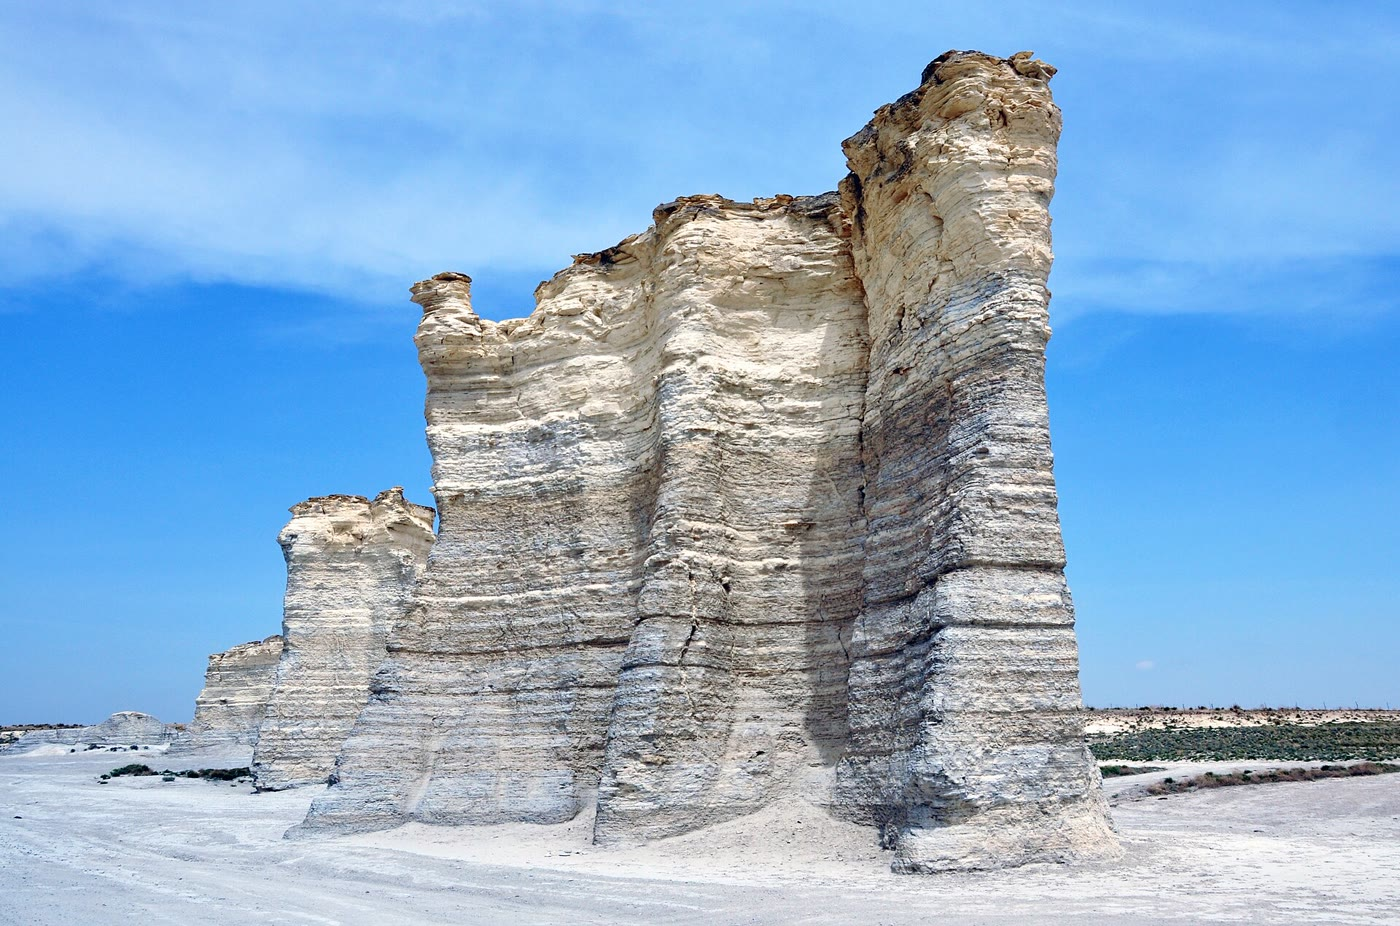
\includegraphics[width=0.66\linewidth]{images/book4/b2-19-monument-rocks.jpg}
\par\smallskip{\small Monument Rocks, western Kansas: pillars of chalk, the ooze of a Cretaceous
inland sea about 80 million years old, laid down at about \qty{0.036}{mm} a year. (James
St.~John, CC~BY~2.0, via Wikimedia Commons.)}
\end{omfigure}
% ledger: kgs:monument-rocks, kgs:chalk

\begin{definition}[Epeiric sea]\label{def:b2:phanerozoic-earth:epeiric}
An \emph{epeiric sea}\index{epeiric sea} is a shallow sea spread over the interior of a
continent, on continental crust, far from the continental margin.
\end{definition}

The sea reaches such interiors by moving its shore, and the rocks record that motion.

\begin{definition}[Marine transgression; marine regression]\label{def:b2:phanerozoic-earth:transgression}
A \emph{marine transgression}\index{marine transgression} is a landward shift of the shoreline,
by which the sea spreads over the land; a \emph{marine regression}\index{marine regression} is
a seaward shift, by which the land emerges.
\end{definition}

In a vertical section, a transgression stacks deeper-water deposits on shallower ones ---
offshore mud over beach sand --- and a regression the reverse. Both follow the relative sea
level, which mixes the global sea level with the subsidence or uplift of the place and with the
supply of sediment: a delta can push its shore seaward while the sea rises, if it is fed fast
enough. To read the global sea level from transgressions, a geologist must find the same signal
on several continents, or remove the subsidence by \omterm{def:b2:basins-compared:backstripping}{backstripping}, as in
\cref{ch:b2:basins-compared}.
% ledger: miller20:rsl

\subsection*{The long-term curve}

\begin{definition}[First-order sea-level cycle]\label{def:b2:phanerozoic-earth:first-order}
The \emph{first-order sea-level cycle}\index{first-order sea-level cycle} is the slowest part of
the change of global sea level, on time scales of tens to hundreds of millions of years, set by
the tectonics of the solid Earth rather than by ice.
\end{definition}

Across the Phanerozoic the first-order curve has the shape of an M: high in the early Palaeozoic,
low while Pangaea assembled and stood, from the Carboniferous to the end of the Triassic, high
again in the Cretaceous, and falling since. Extrapolated from North America, the flood of the Late
Ordovician alone suggests a further rise of 100 to \qty{200}{m}.
Faster changes ride on this curve: those driven by ice are recorded on time scales of $10^4$ to
$10^6$ years, and the Antarctic ice sheet, from about \qty{33.5}{Ma}, moved the sea by 50 to
\qty{60}{m}.
% ledger: th23:flooding, miller11:greenhouse, miller05:abstract

\begin{omfigure}
\centering
% figdata/bachelor-2/phanerozoic.py parts sealevel-haq, sealevel-haqlt, sealevel-kominz, sealevel-kominzlt
\begin{tikzpicture}
\begin{axis}[width=0.92\linewidth, height=6.2cm, x dir=reverse, xmin=0, xmax=252,
  ymin=-130, ymax=280, xlabel={age (\unit{Ma})}, ylabel={sea level above today (\unit{m})},
  xtick={0,50,...,250}, ytick={-100,-50,...,250}, xtick pos=bottom, ytick pos=left,
  tick label style={font=\scriptsize}, label style={font=\small},
  legend style={at={(0.5,1.04)}, anchor=south, draw=none, font=\scriptsize, legend columns=2,
  /tikz/every even column/.append style={column sep=8pt}}]
\addplot[black!30, line width=0.3pt] table[x=age_ma, y=sl_m]
  {figdata/out/bachelor-2-phanerozoic-sealevel-haq.dat};
\addlegendentry{Haq and others (1987)}
\addplot[omThm, line width=0.3pt] table[x=age_ma, y=sl_m]
  {figdata/out/bachelor-2-phanerozoic-sealevel-kominz.dat};
\addlegendentry{New Jersey, backstripped}
\addplot[black, line width=1.2pt] table[x=age_ma, y=sl_m]
  {figdata/out/bachelor-2-phanerozoic-sealevel-haqlt.dat};
\addlegendentry{Haq, 10-Myr mean}
\addplot[omThm!70!black, line width=1.2pt] table[x=age_ma, y=sl_m]
  {figdata/out/bachelor-2-phanerozoic-sealevel-kominzlt.dat};
\addlegendentry{New Jersey, 10-Myr mean}
\addplot[black!50, line width=0.3pt, forget plot] coordinates {(0,0) (252,0)};
\foreach \a/\b/\c in {251.902/201.4/icsTriassic, 201.4/143.1/icsJurassic,
  143.1/66/icsCretaceous, 66/23.04/icsPaleogene, 23.04/2.58/icsNeogene, 2.58/0/icsQuaternary} {
  \edef\tmp{\noexpand\fill[\c] (axis cs:\a,-130) rectangle (axis cs:\b,-112);}\tmp}
\node[font=\tiny, text=white] at (axis cs:226.7,-121) {Triassic};
\node[font=\tiny, text=white] at (axis cs:172.3,-121) {Jurassic};
\node[font=\tiny] at (axis cs:104.6,-121) {Cretaceous};
\node[font=\tiny] at (axis cs:44.5,-121) {Paleogene};
\node[font=\tiny] at (axis cs:12.8,-121) {Neog.};
\end{axis}
\end{tikzpicture}
\par\smallskip{\small Global sea level since \qty{250}{Ma}, as tabulated by Miller and others
(2005): the cycle chart of Haq and others (1987) from the stratigraphy of many basins, and the
sea level backstripped from coreholes of New Jersey, with estimated lowstands (Kominz and
others 2008). Thick lines: 10-Myr running means, the first-order trend. Ages on the 2012 time
scale; the bar at the bottom shows the periods.}
\end{omfigure}
% ledger: data:b4-sealevel, haq87:charts, kominz08:long-term, ics:base.Triassic, ics:base.Jurassic, ics:base.Cretaceous, ics:base.Paleogene, ics:base.Neogene, ics:base.Quaternary, ics:colour.Triassic, ics:colour.Jurassic, ics:colour.Cretaceous, ics:colour.Paleogene, ics:colour.Neogene, ics:colour.Quaternary

The two curves above agree on the shape and disagree on the size. The cycle chart, built from
the stacking of sediments in many basins, puts the long-term sea level of the mid-Cretaceous
about \qty{233}{m} above today's; the New Jersey wells, backstripped one by one, give about
\qty{70}{m} in the Late Cretaceous and a maximum near \qty{110}{m} in the Eocene. Miller and his
colleagues conclude that the long-term Cretaceous peak was $100 \pm \qty{50}{m}$, and that the
cycle charts, right about the timing of the falls, exaggerate their amplitudes. Even New Jersey
is not a perfect gauge: its Late Cretaceous sea is 100 to \qty{150}{m} lower than the volume of
the ocean basins predicts, a gap that the sinking of the region above the subducted Farallon
plate --- dynamic topography --- could explain.
% ledger: data:b4-sealevel, miller05:abstract, kominz08:long-term, miller20:epr

\subsection*{Why the sea moves: ridges}

What raises the sea by a hundred metres for tens of millions of years? Not ice: the Cretaceous
was a warm world with at most small, short-lived ice sheets. The leading answer is the volume of
the ocean ridges. Young ocean floor is hot and stands high; the faster the plates spread, the
younger the floor is on average, the shallower the ocean basins, and the more water spills onto
the continents.
% ledger: miller11:greenhouse, th23:pitman

\begin{proposition}[Sea level and spreading rate]\label{prop:b2:phanerozoic-earth:ridge}
Let ocean floor of area $A_{\text{f}}$ be made at ridges of total length $L$ at the full
spreading rate $u$, and be destroyed at the age $\tau = A_{\text{f}}/(Lu)$, every age between 0
and $\tau$ covering the same area. Let its depth follow the law $d(t) = d_{\text{r}} + c\sqrt t$.
\begin{enumerate}
  \item The mean depth of the floor is $\bar d = d_{\text{r}} + \tfrac23 c\sqrt\tau$.
  \item If the spreading rate becomes $fu$, with $A_{\text{f}}$ and $L$ unchanged, the mean
        depth decreases by $\Delta\bar d = \tfrac23 c\sqrt\tau\,\bigl(1 - f^{-1/2}\bigr)$.
  \item If the floor sinks isostatically under the added water, and the sea does not spread
        over the land, the sea level over an ocean of area $A_{\text{o}}$ rises by
        \[
        \Delta s = \frac{\rho_{\text{m}} - \rho_{\text{w}}}{\rho_{\text{m}}}\,
        \frac{A_{\text{f}}}{A_{\text{o}}}\,\Delta\bar d ,
        \]
        with $\rho_{\text{m}}$ the density of the mantle and $\rho_{\text{w}}$ that of sea water.
\end{enumerate}
\end{proposition}

\begin{proof}
(1) Ridges make new floor at the rate $Lu$ (area per unit time), and every strip of floor lives
for the time $\tau$; in a steady state the area of floor aged between $t$ and $t + \mathrm{d}t$
is $Lu\,\mathrm{d}t$ for every $t < \tau$, so the total area is $Lu\tau = A_{\text{f}}$ and the
ages are evenly spread. The mean depth is
$\frac1\tau\int_0^\tau (d_{\text{r}} + c\sqrt t)\,\mathrm{d}t = d_{\text{r}} + \frac{c}{\tau}
\cdot\frac23\tau^{3/2}$. (2) With the rate $fu$, $\tau$ becomes $\tau/f$, and
$\sqrt{\tau/f} = f^{-1/2}\sqrt\tau$. (3) The basins lose the volume $\Delta V = A_{\text{f}}
\Delta\bar d$. Let the sea surface rise by $\Delta s$ relative to the continents, and the floor
sink by $y$ under the extra water. The extra water column, $\Delta s + y$ thick, replaces a
thickness $y$ of mantle in the isostatic balance: $\rho_{\text{w}}(\Delta s + y) =
\rho_{\text{m}} y$, so $y = \rho_{\text{w}}\Delta s/(\rho_{\text{m}} - \rho_{\text{w}})$ and
$\Delta s + y = \Delta s\,\rho_{\text{m}}/(\rho_{\text{m}} - \rho_{\text{w}})$. Volume is
conserved: $A_{\text{o}}(\Delta s + y) = \Delta V$, which gives the result.
\end{proof}

The real floor is not so tidy. Its ages are not evenly spread: young floor is the most abundant,
and the area falls with age, as the left panel below shows. Nor does the square-root law hold for
old floor, which flattens near \qty{6.4}{km}; the exponential law that Parsons and Sclater
fitted to old floor, the plate law, takes over beyond about \qty{26}{Myr}, where the two laws
meet. The proposition is a first estimate, and the figure
shows how much the second law changes it.
% ledger: ps77:depth-age, data:b4-ridge

\begin{omfigure}
\centering
% figdata/bachelor-2/phanerozoic.py parts agehist and ridge
\begin{tikzpicture}
\begin{groupplot}[group style={group size=2 by 1, horizontal sep=1.6cm},
  width=0.5\linewidth, height=5.6cm, tick label style={font=\scriptsize},
  label style={font=\small}, xtick pos=bottom, ytick pos=left]
\nextgroupplot[xmin=0, xmax=200, ymin=0, ymax=34, xlabel={age of the floor (\unit{Myr})},
  ylabel={area per \qty{10}{Myr} (\unit{\mega km^2})},
  legend style={at={(0.5,1.04)}, anchor=south, draw=none, font=\scriptsize}]
\addplot[ybar interval, area legend, fill=omSea!80!black, draw=black!50, line width=0.2pt]
  table[x expr=\thisrow{age}-5, y=area_Mkm2] {figdata/out/bachelor-2-phanerozoic-agehist.dat};
\addlegendentry{age grid}
\addplot[const plot mark mid, black, dashed, line width=0.9pt]
  table[x=age, y=uniform_Mkm2] {figdata/out/bachelor-2-phanerozoic-agehist.dat};
\addlegendentry{even ages to \qty{128.4}{Myr}}
\nextgroupplot[xmin=1, xmax=3, ymin=0, ymax=650, xlabel={spreading rate / today's, $f$},
  ylabel={sea-level rise $\Delta s$ (\unit{m})},
  legend style={at={(0.5,1.04)}, anchor=south, draw=none, font=\scriptsize, legend columns=2}]
\fill[omThm!15] (axis cs:1,50) rectangle (axis cs:3,150);
\addplot[black, line width=1pt] table[x=f, y=ds_hs] {figdata/out/bachelor-2-phanerozoic-ridge.dat};
\addlegendentry{$\sqrt t$ law}
\addplot[blue!70!black, dashed, line width=1pt] table[x=f, y=ds_plate]
  {figdata/out/bachelor-2-phanerozoic-ridge.dat};
\addlegendentry{plate law}
\node[font=\scriptsize, anchor=west] at (axis cs:1.6,100) {$100 \pm \qty{50}{m}$};
\end{groupplot}
\end{tikzpicture}
\par\smallskip{\small Left: area of today's ocean floor in 10-Myr age bins, from the age grid
of Seton and others (2020) at one-degree resolution (\qty{293}{\mega km^2} in all), against the
even spread of \cref{prop:b2:phanerozoic-earth:ridge} with the same area and mean age. Right:
sea-level rise when the spreading rate is multiplied by $f$, from the proposition with the
square-root law and with the plate law, starting from the even spread to \qty{128.4}{Myr}; the
band is the long-term Cretaceous peak estimated by Miller and others (2005).}
\end{omfigure}
% ledger: data:b4-ridge, data:b2-seafloor-age, seton:mean-age, ps77:depth-age, miller05:abstract, charette:ocean-volume, katz03:thermo, noaa:seawater-1025

\begin{example}[Twice as fast]\label{ex:b2:phanerozoic-earth:doubling}
Take the floor today: mean age \qty{64.2}{Myr}, so $\tau = \qty{128.4}{Myr}$ in the even model;
$d_{\text{r}} = \qty{2500}{m}$, $c = \qty{350}{m.Myr^{-1/2}}$. The mean depth is $2500 + \tfrac23
\times 350 \times \sqrt{128.4} = \qty{5144}{m}$. Doubling the rate halves $\tau$, and the mean
depth becomes $2500 + \tfrac23 \times 350 \times \sqrt{64.2} = \qty{4370}{m}$: the floor rises by
\qty{774}{m} on average. With $A_{\text{f}}/A_{\text{o}} = 293/362 = 0.810$ and
$(\rho_{\text{m}} - \rho_{\text{w}})/\rho_{\text{m}} = (3300 - 1025)/3300 = 0.689$, the sea rises
by $0.689 \times 0.810 \times 774 = \qty{432}{m}$; with the plate law, \qty{368}{m}. Both are
about four times the long-term Cretaceous peak. Read the other way, the right panel says that a
spreading rate only 15 to \qty{20}{\percent} above today's suffices for \qty{100}{m} --- which is
why Miller and his colleagues conclude that ocean crust was made much more slowly in the
Cretaceous than once inferred.
\end{example}
% ledger: seton:mean-age, ps77:depth-age, data:b4-ridge, charette:ocean-volume, katz03:thermo, noaa:seawater-1025, miller05:abstract
% values (phanerozoic.py numbers): dbar_hs 5144, dbar_hs_half 4369.6, rise2_hs 432.5, rise2_pl 368.4, f_for_100_hs 1.151

The model is also too deep: its mean depth, \qty{5144}{m}, exceeds the measured mean depth of
the dated floor, \qty{4265}{m}, partly because the square-root law overshoots on old floor, and
partly because the real floor carries sediment, \omterm{def:b2:oceanic-islands:seamount}{seamounts} and plateaus that the law leaves out. And spreading is not the
only lever. Ridges are balanced by trenches: if the ocean floor rises in one place, the mass must
go somewhere, and a continent sinking over a slab --- dynamic topography --- lets the sea in
locally. Tasistro-Hart and Macdonald argue that the floods of North America follow the slabs
under the continent, and that the global sea level depends on how much subduction happens under
continents rather than under oceans.
% ledger: data:b4-floor-depth, th23:pitman, th23:flooding, kominz08:long-term

\section{Flooding the continents}\label{sec:b2:phanerozoic-earth:flooding}

How much land a rise of the sea drowns depends on the shape of the Earth's surface, which the
hypsometric curve of the Year~1 volume summarises: the fraction of the surface that stands above
each elevation (figure below, left). The continents are flat-topped. On the one-degree grid of
ETOPO1, \qty{29.0}{\percent} of the surface is land and \qty{34.3}{\percent} stands above
\qty{-200}{m}: the shelves, already under water, make the difference. Most land is low, so a
modest rise floods a great deal of it.
% ledger: data:b4-hyps, data:etopo1

\begin{proposition}[Flooding the land]\label{prop:b2:phanerozoic-earth:flooding}
Let $A_{\text{o}}$ be the area of the sea today and $a(z)$ the area of land lower than $z$ above
today's sea level. A volume $V$ of water added to the sea raises its level by the height $s$
that solves
\[
V = \int_0^s \bigl(A_{\text{o}} + a(z)\bigr)\,\mathrm{d}z ,
\]
and floods the land area $a(s)$. Since $a \ge 0$, the rise is at most $V/A_{\text{o}}$.
\end{proposition}

\begin{proof}
When the sea stands at $z$, it covers $A_{\text{o}} + a(z)$; raising it by $\mathrm{d}z$ takes
the volume $\bigl(A_{\text{o}} + a(z)\bigr)\mathrm{d}z$. Summing from 0 to $s$ gives $V$. The
integrand is at least $A_{\text{o}}$, so $V \ge A_{\text{o}}s$.
\end{proof}

\begin{omfigure}
\centering
% figdata/bachelor-2/phanerozoic.py parts hyps and flood
\begin{tikzpicture}
\begin{groupplot}[group style={group size=2 by 1, horizontal sep=1.6cm},
  width=0.46\linewidth, height=5.6cm, tick label style={font=\scriptsize},
  label style={font=\small}, xtick pos=bottom, ytick pos=left]
\nextgroupplot[xmin=0, xmax=100, ymin=-9500, ymax=6500,
  xlabel={per cent of the surface above $z$}, ylabel={elevation $z$ (\unit{m})},
  scaled y ticks=false, yticklabel style={/pgf/number format/1000 sep={\,}}]
\addplot[omThm, line width=1pt] table[x=pct, y=z] {figdata/out/bachelor-2-phanerozoic-hyps.dat};
\addplot[black!50, line width=0.3pt] coordinates {(0,0) (100,0)};
\node[font=\scriptsize, anchor=south west] at (axis cs:30,100) {land \qty{29.0}{\percent}};
\node[font=\scriptsize] at (axis cs:45,-7000) {ocean floor};
\nextgroupplot[xmin=0, xmax=1000, ymin=0, ymax=80, xlabel={sea-level rise $h$ (\unit{m})},
  ylabel={land flooded (\unit{\percent})}]
\addplot[omThm, line width=1pt] table[x=h, y=flooded_pct]
  {figdata/out/bachelor-2-phanerozoic-flood.dat};
\addplot[black, dashed, line width=0.5pt] coordinates {(100,0) (100,14.9) (0,14.9)};
\addplot[black, dashed, line width=0.5pt] coordinates {(432,0) (432,50.6) (0,50.6)};
\end{groupplot}
\end{tikzpicture}
\par\smallskip{\small Left: hypsometric curve of the Earth from the one-degree ETOPO1 grid.
Right: per cent of today's land below each height above sea level, the land a rise $h$ would
flood if nothing else moved; the dashed lines mark \qty{100}{m} and \qty{432}{m}. Averaging over
one-degree cells smooths the relief, so these are first estimates.}
\end{omfigure}
% ledger: data:b4-hyps, data:etopo1

The right panel gives the answer at once. A rise of \qty{100}{m} drowns about
\qty{15}{\percent} of today's land; the \qty{432}{m} of a doubled spreading rate would drown
half. Such a sea spreads over the land it floods, so the rise itself is smaller than the
proposition's bound $V/A_{\text{o}}$, by about a tenth for a rise of a few hundred metres (weekend
problem). The Cretaceous seas of Kansas needed far less: the interior of a continent is often
low, and it may also sink over a slab.
% ledger: data:b4-hyps
% values (phanerozoic.py numbers): flood_100 14.9, flood_rise2 50.8, level_rise2_spread 390.7

\section{Mountain belts of the Phanerozoic}\label{sec:b2:phanerozoic-earth:orogens}

Each \omterm{def:b2:wilson-cycle:wilson}{Wilson cycle} of \cref{ch:b2:wilson-cycle} ends in a mountain belt, and the Phanerozoic
belts mark the making and the breaking of Pangaea. The table gathers those met in this volume.

\begin{center}
\small
\begin{tabular}{>{\raggedright\arraybackslash}p{0.15\linewidth}>{\raggedright\arraybackslash}p{0.22\linewidth}>{\raggedright\arraybackslash}p{0.22\linewidth}>{\raggedright\arraybackslash}p{0.29\linewidth}}
\hline
orogeny & time & ocean closed & what met \\
\hline
Caledonian & c.~540--400 Ma; main collision 425--400 Ma & Iapetus & Laurentia, Baltica and
Avalonia, forming Laurussia \\
Variscan--Appalachian & from c.~550 Ma; final collision Late Carboniferous--Permian & Rheic &
Gondwana and its detached \omterm{def:b2:wilson-cycle:terrane}{terranes} with Laurussia, forming Pangaea \\
Alpine & Cretaceous (peak near 100 Ma) and Cenozoic & Alpine Tethys & Apulia and Europe \\
Himalayan & from c.~60 to 54 Ma (debated) to today & ocean north of India & India and Asia \\
Andean & still active; shortening since the Oligocene & none: an ocean plate subducts & the
Nazca plate beneath South America \\
\hline
\end{tabular}
\end{center}
% ledger: mckerrow00:caledonian, schiffer20:caledonides, schiffer20:variscan, faure24:variscan, usgs:alleghanian-age, schmid04:two-orogenies, najman21:collision-age, gerbault05:andes, nance22:supercontinents

The first two belts sewed Pangaea together, the Variscan closing the last ocean between Gondwana
and Laurussia; the last three grew as the pieces of Pangaea moved apart and the oceans between
them were consumed. The low sea level of the late Palaeozoic and Triassic belongs to this
\omterm{def:b2:wilson-cycle:supercontinent}{supercontinent}, and the high sea of the Cretaceous to its break-up, with new ridges and young
floor.
% ledger: schiffer20:variscan, th23:flooding, nance22:supercontinents

\section{Crises of life}\label{sec:b2:phanerozoic-earth:extinctions}

\subsection*{The big five}

The biology volumes describe mass extinctions; geologists measure them in the rocks and look for
their causes. Five stand out in the record of marine animals, the ``big five'': at the end of the
Ordovician, about \qty{444}{Ma}; in the Late Devonian, \qty{372}{Ma}; at the end of the Permian,
\qty{251.9}{Ma}; at the end of the Triassic, \qty{201.4}{Ma}; and at the end of the Cretaceous,
\qty{66}{Ma}. Each removed between about two fifths and two thirds of the genera of marine
animals in Sepkoski's compilation. The end-Permian crisis was the largest: \qty{56}{\percent} of
genera at the finest resolution, and about \qty{81}{\percent} of marine species --- not the
\qty{96}{\percent} often quoted, which mixed two separate crises.
% ledger: kaiho22:table, marshall23:big-five, stanley16:permian

\begin{history}[The big five, forty years on]
In 1982, D.~M.~Raup and J.~J.~Sepkoski counted the families of marine animals that disappeared
in each of 76 stages of the Phanerozoic. Four points stood above the 99~per cent confidence limit
of their trend --- the last stage of the Ordovician, the last two of the Permian and the last of
the Cretaceous --- and the end of the Triassic and the end of the Devonian above the 95~per cent
limit: the big five. Forty years later, the five remain the largest crises since the early
Ordovician, but with better data they no longer stand apart from a continuum of extinction
rates, and some intervals of the Cambrian had even higher rates. Raup and Sepkoski's time
resolution was \qty{7.4}{Myr}, the mean length of a stage then; some crises were sudden, others
lasted hundreds of thousands of years or longer.
\end{history}
% ledger: marshall23:big-five, marshall23:resolution

\begin{omfigure}
\centering
% figdata/bachelor-2/phanerozoic.py parts ext, lip, oae
\begin{tikzpicture}
\begin{axis}[width=0.95\linewidth, height=6.4cm, x dir=reverse, xmin=0, xmax=541,
  ymin=-34, ymax=80, xlabel={age (\unit{Ma})}, ylabel={marine genera lost (\unit{\percent})},
  xtick={0,100,...,500}, ytick={0,20,...,80}, xtick pos=bottom, ytick pos=left,
  tick label style={font=\scriptsize}, label style={font=\small}, clip=false]
\addplot[ybar, bar width=5pt, fill=omThm!70, draw=black!60, point meta=explicit symbolic,
  nodes near coords, nodes near coords style={font=\tiny, anchor=south}]
  table[x=age, y=value, meta=label] {figdata/out/bachelor-2-phanerozoic-ext.dat};
\addplot[only marks, mark=triangle*, mark size=2.6pt, red!70!black]
  table[x=age, y expr=-6] {figdata/out/bachelor-2-phanerozoic-lip.dat};
\addplot[only marks, mark=diamond*, mark size=2.6pt, blue!70!black]
  table[x=age, y expr=-13] {figdata/out/bachelor-2-phanerozoic-oae.dat};
\addplot[only marks, mark=star, mark size=4pt, line width=1pt, black] coordinates {(66,-20)};
\node[font=\tiny, anchor=west, red!70!black] at (axis cs:541,-6) {LIPs};
\node[font=\tiny, anchor=west, blue!70!black] at (axis cs:541,-13) {OAEs};
\node[font=\tiny, anchor=west] at (axis cs:541,-20) {impact};
\node[font=\tiny, anchor=west] at (axis cs:57,-20) {Chicxulub};
\foreach \a/\b/\c in {538.8/486.85/icsCambrian, 486.85/443.1/icsOrdovician,
  443.1/419.62/icsSilurian, 419.62/358.86/icsDevonian, 358.86/298.9/icsCarboniferous,
  298.9/251.902/icsPermian, 251.902/201.4/icsTriassic, 201.4/143.1/icsJurassic,
  143.1/66/icsCretaceous, 66/23.04/icsPaleogene, 23.04/2.58/icsNeogene, 2.58/0/icsQuaternary} {
  \edef\tmp{\noexpand\fill[\c] (axis cs:\a,-34) rectangle (axis cs:\b,-27);}\tmp}
\foreach \x/\t in {512.8/Cm, 465/O, 431.4/S, 389.2/D, 328.9/C, 275.4/P, 226.7/Tr, 172.3/J,
  104.6/K, 44.5/Pg, 12.8/N} {
  \edef\tmp{\noexpand\node[font=\noexpand\tiny] at (axis cs:\x,-30.5) {\t};}\tmp}
\end{axis}
\end{tikzpicture}
\par\smallskip{\small The big five mass extinctions, with the share of marine genera lost in
Sepkoski's compilation (Kaiho 2022, Table~1), large igneous provinces (triangles, mean ages of
Courtillot and Renne 2003, from \qty{259}{Ma}), the best-studied \omterm{def:b2:phanerozoic-earth:oae}{oceanic anoxic events}
(diamonds) and the Chicxulub impact. The bar at the bottom shows the periods.}
\end{omfigure}
% ledger: kaiho22:table, cr03:table, rigo24:oaes, pickersgill26:chicxulub, ics:base.Cambrian, ics:base.Ordovician, ics:base.Silurian, ics:base.Devonian, ics:base.Carboniferous, ics:base.Permian, ics:base.Triassic, ics:base.Jurassic, ics:base.Cretaceous, ics:base.Paleogene, ics:base.Neogene, ics:base.Quaternary, ics:colour.Cambrian, ics:colour.Ordovician, ics:colour.Silurian, ics:colour.Devonian, ics:colour.Carboniferous, ics:colour.Permian

\subsection*{Large igneous provinces}

The figure above shows the pattern that the Year~1 volume pointed to: the three most recent of
the big five each fall on a large igneous province, the Siberian Traps at the end of the Permian,
the Central Atlantic Magmatic Province (CAMP) at the end of the Triassic, the Deccan Traps at the
end of the Cretaceous. The proposed link is the gas. A flood basalt erupts in pulses of a few
centuries to a few millennia, each releasing carbon dioxide faster than weathering can take it
back; the sulfur of the same eruptions cools the climate briefly, the carbon warms it for much
longer and acidifies the ocean.
% ledger: cr03:table, cr03:summary, capriolo20:camp-co2

\begin{example}[The carbon of the Central Atlantic province]\label{ex:b2:phanerozoic-earth:camp}
Gas bubbles in melt inclusions of CAMP basalts show that the \omterm{def:b2:magma-emplacement:magma}{magma} held at least 0.5 to
\qty{0.6}{\percent} of carbon dioxide by mass. Take \qty{0.55}{\percent}, a density of
\qty{2900}{kg.m^{-3}} and a volume of \qty{5.5e6}{km^3}, the erupted lavas with the \omterm{def:b2:magma-emplacement:bodies}{dykes}, \omterm{def:b2:magma-emplacement:bodies}{sills}
and chambers that fed them. The mass of \omterm{def:b2:magma-emplacement:magma}{magma} is $\num{5.5e6} \times \num{e9} \times 2900 =
\qty{1.6e19}{kg}$, and its carbon dioxide $\num{1.6e19} \times 0.0055 = \qty{8.8e16}{kg}$, about
\qty{9e4}{Gt} --- the authors' ``up to \qty{e5}{Gt}''. Released over the province's lifetime, it
was not all in the air at once; but each pulse, of the order of \qty{e5}{km^3} in a few
centuries, released as much as the emissions projected for the twenty-first century.
\end{example}
% ledger: capriolo20:camp-co2
% values: 5.5e6 km3 x 2900 kg/m3 = 1.595e19 kg; x 0.0055 = 8.77e16 kg

\subsection*{Oceanic anoxic events}

Not every crisis is one of the big five. Several times in the Mesozoic, oxygen disappeared from
large parts of the ocean.

\begin{definition}[Oceanic anoxic event]\label{def:b2:phanerozoic-earth:oae}
An \emph{oceanic anoxic event}\index{oceanic anoxic event} (OAE) is an interval of widespread
oxygen depletion in the ocean, recognised in the sedimentary and geochemical record.
\end{definition}

Its usual mark is a black shale: dark, finely laminated, without burrows, rich in organic matter
and in pyrite, often with a shift of the carbon isotopes and signs of warming. The best studied
are the early Toarcian event, about \qty{183}{Ma}, the early Aptian OAE~1a, about \qty{120}{Ma},
the early Albian OAE~1b, about \qty{111}{Ma}, and OAE~2 at the boundary between the Cenomanian
and the Turonian, about \qty{94}{Ma}, in the hottest part of the Cretaceous, when the sea stood
exceptionally high. Several coincide with a province: the Toarcian event with the Karoo--Ferrar
basalts, OAE~1a with the Ontong Java Plateau. OAE~2 is often tied to the Caribbean plateau, but
mercury spikes in Southern Hemisphere sediments point to the Kerguelen province instead.
% ledger: rigo24:oaes, wt24:oae2, cr03:table

\begin{omfigure}
\centering
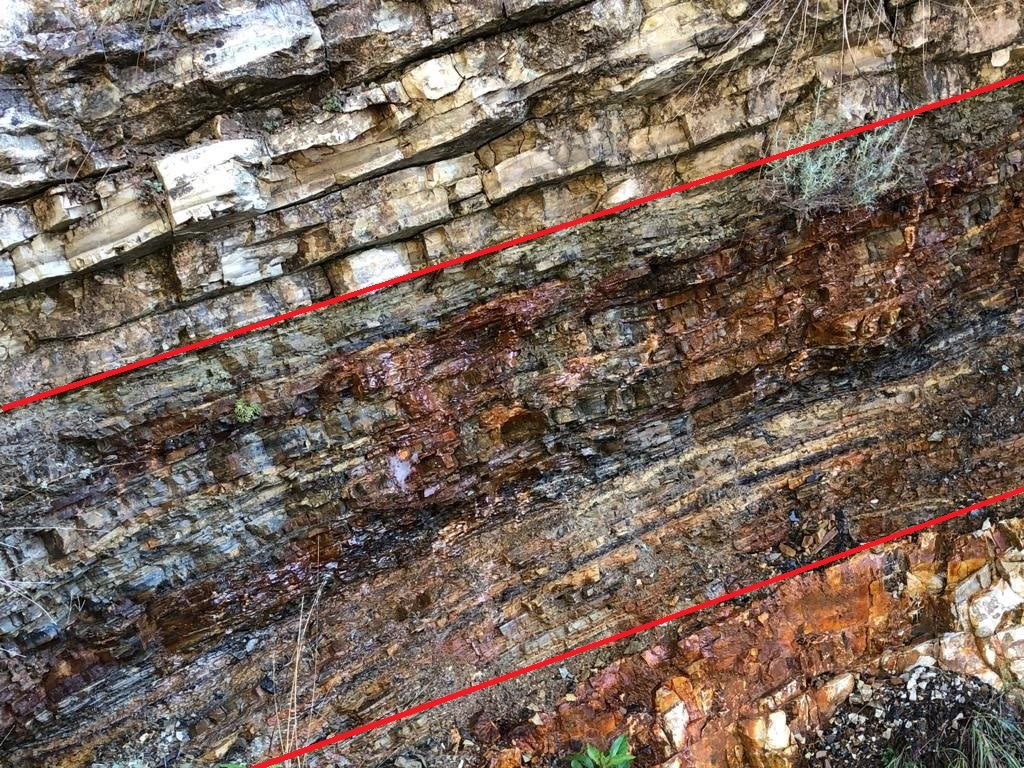
\includegraphics[width=0.66\linewidth]{images/book4/b2-19-bonarelli-level.jpg}
\par\smallskip{\small The Bonarelli level, the dark shale of OAE~2, between pale limestones; the
red lines, drawn by the photographer, mark its base and top. (Picenus, CC~BY-SA~4.0, via
Wikimedia Commons.)}
\end{omfigure}
% ledger: rigo24:oaes

\begin{inthefield}[Logging an anoxic event]
A geologist who studies an OAE in a section of pelagic limestones logs it bed by bed: thickness,
colour, lamination, burrows or their absence, nodules of pyrite. She samples at close, regular
intervals across the dark interval and well beyond it, for the organic carbon content and for the
carbon isotopes of the organic matter and of the carbonate; the shift of the isotopes, more than
the colour of the rock, correlates the event from one basin to the next. Because the darkest
shale can appear at different levels in different basins, the isotope curve, not the black
shale, is taken as the time line.
\end{inthefield}
% ledger: rigo24:oaes, wt24:oae2

\subsection*{Chicxulub}

The end of the Cretaceous had a cause from outside. The Year~1 volume told how the iridium of the
boundary clay led to an impact, and how argon dating tied the boundary to the Chicxulub crater.
The structure is about \qty{200}{km} across and \qty{66}{Ma} old; its
hot rocks fed circulating water for at least eight million years after. Models of its subsurface
asymmetry point to an impactor that came from the north-east at 45 to \ang{60} to the horizontal,
at no less than the Earth's escape velocity, \qty{11.2}{km.s^{-1}}, and more probably about
\qty{20}{km.s^{-1}}. The Deccan Traps were erupting at the same time, before and after the
impact; a review of the evidence in 2010 concluded that the impact triggered the extinction.
% ledger: pickersgill26:chicxulub, collins20:impact, renne:kpg, alvarez:iridium, schulte:kpg, cr03:deccan

\begin{dated}{2026}
The ages in this chapter are those of the International Chronostratigraphic Chart in its June
2026 version, as used throughout this series; the sea-level records are on the 2012 time scale
of their files, and the extinction ages are those of Kaiho (2022). The chart is revised as new
dates come in: check the current version before quoting a boundary age.
\end{dated}
% ledger: ics:base.Phanerozoic, data:b4-sealevel, kaiho22:table

\section*{Exercises}\label{sec:b2:phanerozoic-earth:exercises}

Data for the exercises, unless stated otherwise: \qty{111.2}{km} per degree of latitude; depth
of the ocean floor $d(t) = 2500 + 350\sqrt t$ (\unit{m}, $t$ in \unit{Myr}); ocean area
\qty{362}{\mega km^2}; ocean floor area \qty{293}{\mega km^2}; mantle density
\qty{3300}{kg.m^{-3}}; sea water \qty{1025}{kg.m^{-3}}; mass of the atmosphere
\qty{5.1e18}{kg}, molar masses of air and of carbon dioxide \qty{28.97}{g.mol^{-1}} and
\qty{44.01}{g.mol^{-1}}.
% ledger: earth:Rmean, ps77:depth-age, charette:ocean-volume, data:b4-ridge, katz03:thermo, noaa:seawater-1025, earth:Matm, earth:Mmol, ciaaw:abridged-2024

\begin{exercise}[$\star$]\label{exo:b2:phanerozoic-earth:1}
In the model of the maps, Cape Town lay at \ang{61.9}~S \qty{300}{Ma} ago and New York at
\ang{3.6}~S; today they lie at \ang{33.9}~S and \ang{40.7}~N. (a) Which of the four cities lay
within \ang{30} of the equator \qty{300}{Ma} ago (Paris at \ang{5.1}~N, Sydney at
\ang{59.5}~S)? (b) How far north, in kilometres, has each of Cape Town and New York moved since?
(c) At what mean rates, in centimetres a year?
\end{exercise}
% ledger: data:b4-palaeopos, geonames4:cities

\begin{exercise}[$\star$]\label{exo:b2:phanerozoic-earth:2}
The big five fell at 444, 372, 251.9, 201.4 and \qty{66}{Ma}. (a) Find the intervals between
successive crises and their mean. (b) Using the mean ages of the large igneous provinces ---
Emeishan 259, Siberian 250, CAMP 201, Karoo--Ferrar 183, Deccan \qty{65.5}{Ma} --- which of the
five fall within \qty{2}{Myr} of a province? (c) Does a mean interval make the crises periodic?
\end{exercise}
% ledger: kaiho22:table, cr03:table

\begin{exercise}[$\star$]\label{exo:b2:phanerozoic-earth:3}
The chalk of Monument Rocks was laid down at about \qty{0.036}{mm} a year. (a) How long did
\qty{91}{m} of it take? (b) How many times faster does the sea rise today, at \qty{3.7}{mm} a
year? (c) Why can a sea floor collect such a slow rain of sediment without being buried by mud?
\end{exercise}
% ledger: kgs:monument-rocks, ipcc:sea-level-obs

\begin{exercise}[$\star$]\label{exo:b2:phanerozoic-earth:4}
In a cliff, from the bottom up: river sandstone with roots, beach sand with shells, grey offshore
mud, chalk; then the chalk is overlain by beach sand again. (a) Where does the section record a
\omterm{def:b2:phanerozoic-earth:transgression}{marine transgression}, and where a regression? (b) Does the transgression prove that global sea
level rose? (c) What would make it more convincing?
\end{exercise}

\begin{exercise}[$\star\star$]\label{exo:b2:phanerozoic-earth:5}
On the long-term curve of Haq and others, sea level stood \qty{233}{m} above today's at
\qty{97}{Ma}. (a) What mean rate of fall since then, in metres per million years and in
micrometres a year? (b) Compare with today's rise of \qty{3.7}{mm} a year. (c) The backstripped
New Jersey curve gives about \qty{70}{m} at the same time. Which would you trust for the
amplitude, and why?
\end{exercise}
% ledger: data:b4-sealevel, ipcc:sea-level-obs, miller05:abstract, miller20:epr

\begin{exercise}[$\star\star$]\label{exo:b2:phanerozoic-earth:6}
A single pulse of the CAMP, about \qty{e5}{km^3} of basalt of density \qty{2900}{kg.m^{-3}},
erupted in about 500 years. (a) With \qty{0.75}{\percent} of carbon dioxide by mass, how much
did it release, in kilograms and in moles? (b) What mass of carbon dioxide did the air hold at
the \qty{278}{ppm} of 1750? (c) Compare. (d) How many such atmospheres would the whole province,
\qty{e5}{Gt}, have provided?
\end{exercise}
% ledger: capriolo20:camp-co2, ipcc:erf-2xco2, earth:Matm, earth:Mmol, ciaaw:abridged-2024

\begin{exercise}[$\star\star$]\label{exo:b2:phanerozoic-earth:7}
Take the Chicxulub impactor as a sphere \qty{10}{km} across, of density
\qty{2630}{kg.m^{-3}}. (a) Find its mass. (b) Find its kinetic energy at the least possible
speed, \qty{11.2}{km.s^{-1}}, and at \qty{20}{km.s^{-1}}. (c) The Earth loses \qty{47}{TW} of
internal heat through its surface. How many years of that loss does each energy represent?
\end{exercise}
% ledger: alvarez:iridium, collins20:impact, b2dd10:half-space

\begin{exercise}[$\star\star$]\label{exo:b2:phanerozoic-earth:8}
(a) List the features by which a black shale records an \omterm{def:b2:phanerozoic-earth:oae}{oceanic anoxic event}. (b) Pair each
event with a province of nearly the same age: early Toarcian, \qty{183}{Ma}; OAE~1a,
\qty{120}{Ma}; given Karoo--Ferrar at \qty{183}{Ma} and Ontong Java at \qty{122}{Ma}. (c) Why is a
coincidence of ages not enough to prove that a province caused an event?
\end{exercise}
% ledger: rigo24:oaes, cr03:table

\begin{exercise}[$\star\star$]\label{exo:b2:phanerozoic-earth:9}
In the model, Paris lay at \ang{60.9}~S \qty{500}{Ma} ago and at \ang{5.1}~N \qty{300}{Ma} ago.
(a) Find its northward displacement in degrees and in kilometres, and the mean rate in
centimetres a year. (b) Compare with the rate since \qty{300}{Ma}
(\cref{ex:b2:phanerozoic-earth:paris}). (c) Why is the rate a minimum?
\end{exercise}
% ledger: data:b4-palaeopos

\begin{exercise}[$\star\star\star$]\label{exo:b2:phanerozoic-earth:10}
Suppose instead that the area of floor falls linearly with age, from a maximum at age 0 to zero
at age $T$. (a) Show that the mean age is $T/3$ and that the mean of $\sqrt t$ is
$\tfrac{8}{15}\sqrt T$. (b) With a mean age of \qty{64.2}{Myr}, find $T$ and the mean depth. (c)
Find the fall of the mean depth when the spreading rate doubles, and compare with the
\qty{774}{m} of the even model. (d) Show that in both models the fall is close to $0.93\,c\sqrt{\bar
t}\,(1 - f^{-1/2})$, with $\bar t$ the mean age.
\end{exercise}

\begin{exercise}[$\star\star\star$]\label{exo:b2:phanerozoic-earth:11}
(a) From \cref{prop:b2:phanerozoic-earth:ridge}, show that $\Delta s(f) = \Delta s(2)\,(1 -
f^{-1/2})/(1 - 2^{-1/2})$. (b) With $\Delta s(2) = \qty{432}{m}$, find the range of $f$ that
gives the Cretaceous peak, 50 to \qty{150}{m}. (c) What would a spreading rate slowed to 0.8 of
today's do? (d) Why is a long-term sea level set by ridges a slow signal, whatever the change of
rate?
\end{exercise}
% ledger: data:b4-ridge, miller05:abstract

\begin{exercise}[$\star\star\star$]\label{exo:b2:phanerozoic-earth:12}
Suppose species die out at a constant rate, so that the fraction of a cohort that survives a time
$t$ is $2^{-t/m}$, with a median species longevity $m = \qty{2}{Myr}$. (a) What fraction of a
cohort is gone after \qty{7.4}{Myr}, the mean stage length of the 1982 analysis? (b) How long
would background extinction take to remove \qty{81}{\percent} of species? (c) The end-Permian
crisis lasted about \qty{60}{kyr}. How much faster was it? (d) Why does a coarse time
resolution blur the difference between a mass extinction and a background one?
\end{exercise}
% ledger: marshall23:resolution, stanley16:permian, burgess:end-permian

\begin{problem}[{Weekend problem --- When the ridges were fast}]\label{pb:b2:phanerozoic-earth:1}
This problem asks how much the sea would rise, and how much land it would drown, if the
ridges spread twice as fast. Use the data of the exercises; the mean age of the ocean floor is
\qty{64.2}{Myr}, the ridges are \qty{65000}{km} long in all, today's ocean holds
\qty{1.33e9}{km^3}, and the land covers \qty{148}{\mega km^2}. The table gives the per cent of
today's land lying less than $h$ above sea level, from the one-degree ETOPO1 grid.
\begin{center}
\small
\begin{tabular}{lcccccc}
\hline
$h$ (\unit{m}) & 0 & 100 & 200 & 300 & 400 & 500 \\
land below $h$ (\unit{\percent}) & 0 & 14.9 & 28.2 & 38.7 & 48.1 & 55.8 \\
\hline
\end{tabular}
\end{center}
Assume, as in \cref{prop:b2:phanerozoic-earth:ridge}, that every age of floor between 0 and the
age $\tau$ at which it is subducted covers the same area.

\noindent\textbf{Part I --- The ocean floor today.}
\begin{enumerate}
  \item Find the depth of the floor at ages 0, 25, 64.2 and \qty{100}{Myr}.
  \item Find $\tau$ from the mean age, and the depth of the oldest floor.
  \item Find the mean full spreading rate $u = A_{\text{f}}/(L\tau)$, in kilometres per million
        years and in millimetres a year. Is it a slow, intermediate or fast rate?
  \item Show that the mean depth of the floor is $2500 + \tfrac23 \times 350\sqrt\tau$, and
        compute it.
  \item The measured mean depth of the dated floor is \qty{4265}{m}. Give two reasons why the
        model is deeper.
  \item What volume of water would lie above the floor in the model? Compare with the volume of
        the whole ocean.
\end{enumerate}

\noindent\textbf{Part II --- A ridge in cross-section.}
\begin{enumerate}[resume]
  \item Find the half spreading rate $v$, to the nearest \qty{0.1}{km.Myr^{-1}}, and the width
        of floor on each side of the ridge.
  \item How deep is the floor \qty{1000}{km} from the axis?
  \item Show that the cross-section of the ridge above the depth of the oldest floor, counting
        both flanks, has the area $\tfrac23 v c\,\tau^{3/2}$, and compute it in
        square kilometres.
  \item Find the volume of the whole ridge system above that depth.
  \item What fraction of the volume of the ocean is that?
  \item Why does a ridge spreading faster stand higher on average?
\end{enumerate}

\noindent\textbf{Part III --- Twice as fast.}
\begin{enumerate}[resume]
  \item The spreading rate doubles with the same floor area and ridge length. Find the new $\tau$
        and the new mean depth.
  \item By how much does the mean depth fall?
  \item What volume of water does the floor push out of the basins?
  \item Spread over today's ocean, how much would it raise the sea?
  \item Include the sinking of the floor under the extra water to find the rise $\Delta s$.
  \item The long-term Cretaceous peak was about \qty{100}{m}. What increase of the spreading rate
        would give that?
\end{enumerate}

\noindent\textbf{Part IV --- The sea over the land.}
\begin{enumerate}[resume]
  \item What area of land would a rise of \qty{100}{m} flood?
  \item What area would a rise of \qty{432}{m} flood, by interpolation in the table?
  \item Why must the sea rise by less than \qty{432}{m} once it spreads over the land?
  \item Find the volume needed to raise the sea in steps of \qty{100}{m} up to \qty{400}{m},
        averaging the flooded area over each step (\cref{prop:b2:phanerozoic-earth:flooding}).
        The volume to place is $\qty{0.432}{km} \times \qty{362}{\mega km^2}$. Where does the
        sea stop?
  \item What per cent of today's land does it then cover?
  \item To sum up: in this model, by how much would doubling the spreading rate raise the sea?
\end{enumerate}
\end{problem}
% ledger: ps77:depth-age, seton:mean-age, seton:rate-classes, noaa:ridge, charette:ocean-volume, data:b4-ridge, data:b4-floor-depth, katz03:thermo, noaa:seawater-1025, data:b4-hyps, miller05:abstract
